\subsection{Rectifier Behavior}\label{sec:rectifier-behavior}
A rectenna receives electromagnetic power via antenna and convert it to electric power with rectifier. Diverse configurations are available for energy harvesting, such as \textit{Schottky} \cite{Akkermans2005, Boaventura2013}, \textit{CMOS} \cite{Stoopman2014, Valenta2014}, \textit{series} \cite{Georgiadis2011, Collado2013}, \textit{shunt} \cite{McSpadden1998, Guo2012}. It is worth noting that those models favor different input power levels. As reported in \cite{Valenta2014, Costanzo2016}, low barrier Schottky diodes are commonly used for input power between \SI{1}{\uW} and \SI{1}{\mW}. Specifically, single diode is preferred for a power below \SI{500}{\uW} while multiple diodes are more suitable for power above \SI{500}{\uW} \cite{Clerckx2019}. Hybrid designs as \cite{Sun2013} may be employed to maintain a high efficiency for a wide power range.

Besides the rectenna model, the shape of the received signal also influences the RF-to-DC efficiency ${e_3}$. It was first demonstrated in \cite{Trotter2009} that multisine waveform i.e. \textit{Power-Optimized waveform} (POW) outperforms the single-tone waveform i.e. \textit{Continuous Wave} (CW) in both operation range and power efficiency. Therefore, multisine is commonly employed in WPT waveform design.

The expression of a multisine waveform with $N$ subcarriers writes as a summation of $N$ sine waves

\begin{equation}\label{eqn:multisine}
  {V_{{\text{multisine}}}}(t) = \sum\limits_{n = 0}^{N - 1} {\frac{1}{{\sqrt N }}} \sin \left( {2\pi \left( {{f_{\text{0}}} + n\Delta f} \right)t} \right)
\end{equation}

where ${{f_{\text{0}}}}$ is the minimum frequency and ${\Delta f}$ is the spacing. Fig. \ref{fig:waveform_comparison} \cite{Trotter2009} illustrates a three-subcarrier multisine and single sine in time and frequency domains. It can be observed that multisine provides a higher PAPR of ${\sqrt N }$ and occupies a bandwidth of $(N - 1) \Delta f$. Compared with the single sine, it has the same average power but equally distributed to the components. The thick lines indicate typical rectifier output voltage.

\begin{figure}[ht]
  \centering
  \subfigure[Frequency domain]{
    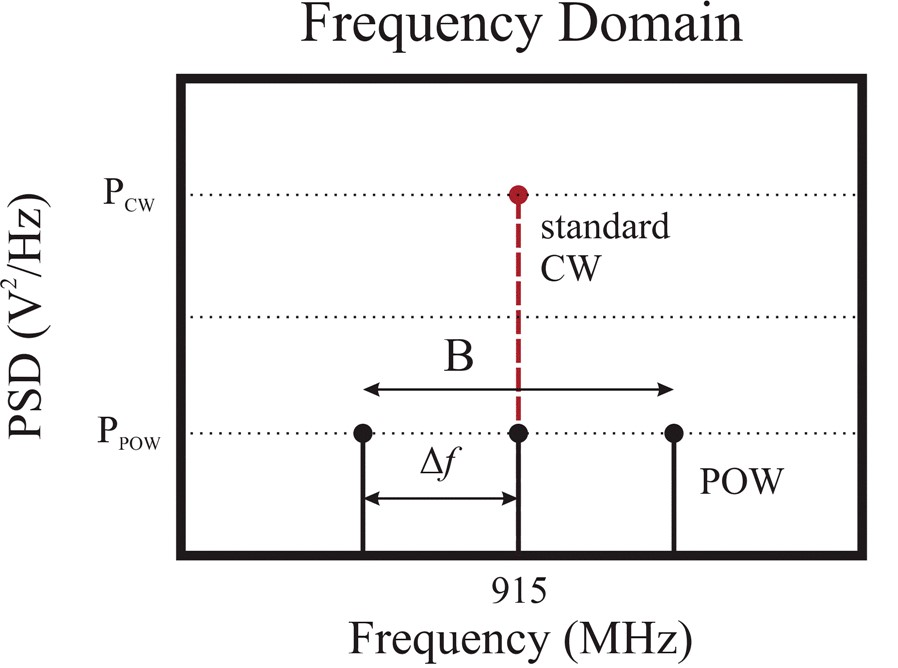
\includegraphics[width=0.48\textwidth]{waveform_frequency_domain}\label{fig:waveform_frequency_domain}}
  \subfigure[Time domain]{
    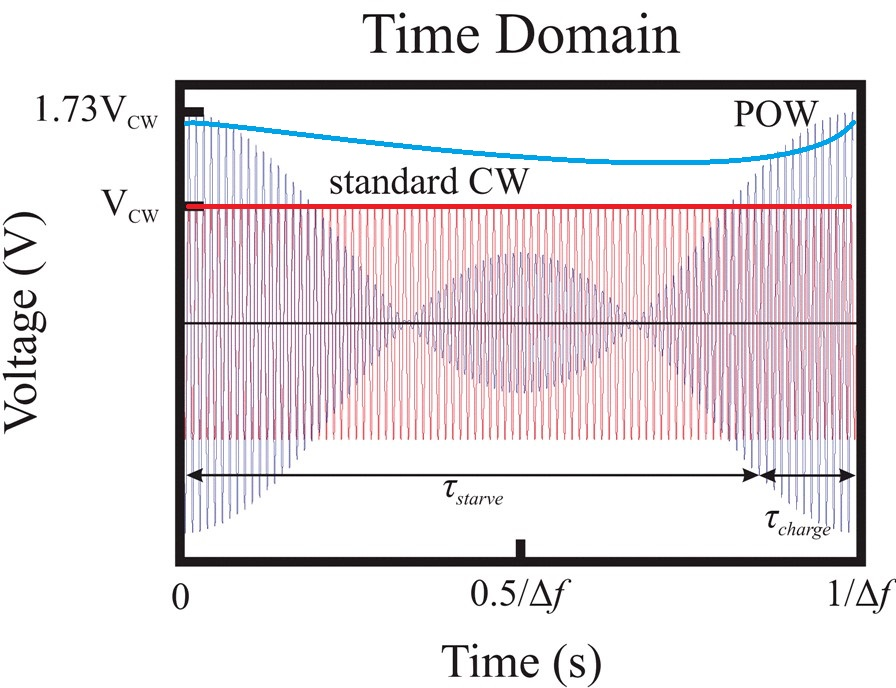
\includegraphics[width=0.48\textwidth]{waveform_time_domain}\label{fig:waveform_time_domain}}
  \caption{A typical 3-subcarrier multisine and single sine \cite{Trotter2009}}
  \label{fig:waveform_comparison}
\end{figure}

The advantage of multisine is that high PAPR can be exploited to increase the peak output voltage of the rectifier. With a proper signal and circuit design, the high output voltage may be preserved during the cycle if discharging is slow enough (as indicated by the thick blue line in Fig. \ref{fig:waveform_time_domain}). To enhance the harvested power, a large number of tones may be used to increase PAPR, and the multisine signal will appear as pulses with a period of $1/\Delta f$. Most of the signal power will be concentrated in those pulses to trigger the diode and charge the capacitor. However, more subbands can lead to smaller frequency gaps and longer charging cycle when the bandwidth is fixed.

It can be hard to derive an accurate expression of the RF-to-DC efficiency ${e_3}$ on the power and shape of the rectifier input signal, as practical energy harvesting circuits consists of various nonlinear components like diodes, capacitors, and inductors. It is also sensitive to parasitic sources, impedance matching, and harmonic generation \cite{Strassner2013, Valenta2014}. In this article, we employ the \textit{diode linear model} and \textit{diode nonlinear model} proposed in \cite{Clerckx2016} based on the diode current-voltage (I-V) characteristics to capture the fundamental pattern of the rectifier and investigate its impact on resource allocation and system design. A superposed waveform containing modulated information and multisine power components is optimized according to CSI on top of both models.



\subsection{Antenna Model}\label{sec:antenna-model}

As illustrated in Fig. \ref{fig:single_diode_rectifier} \cite{Clerckx2016}, the rectifier consists of a single diode as the source of nonlinearity and a low-pass filter to store energy.

\begin{figure}[ht]
  \centering
  \subfigure[A single diode rectifier]{
    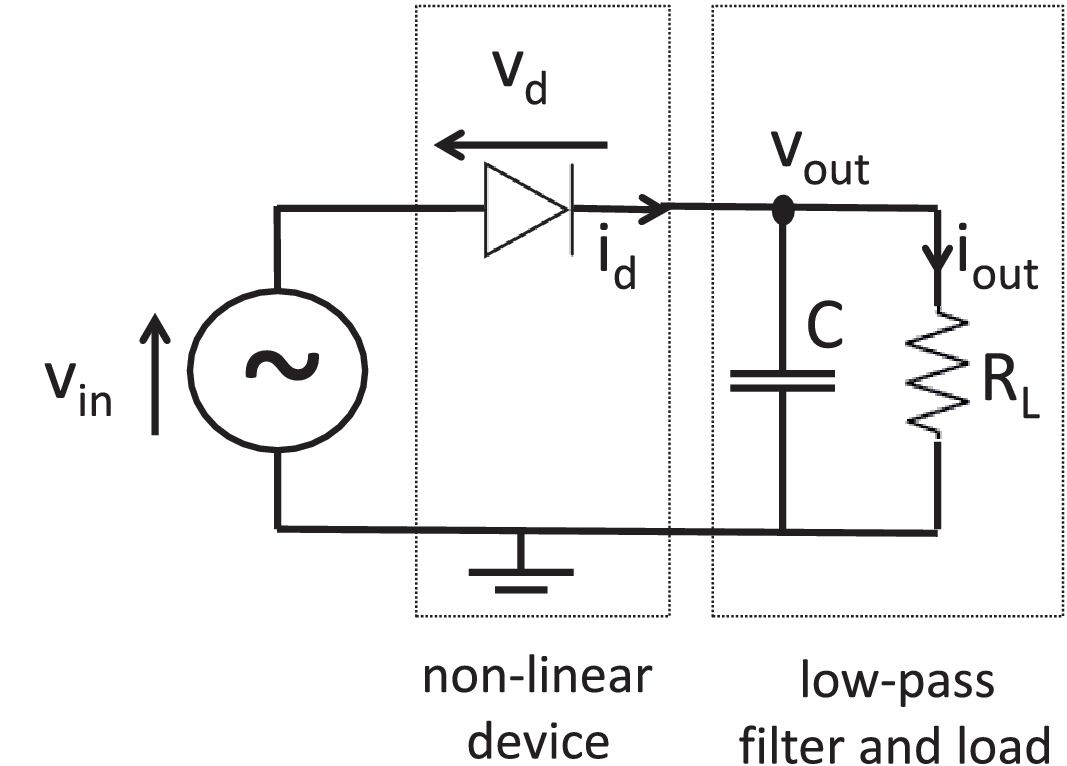
\includegraphics[width=0.48\textwidth]{single_diode_rectifier}\label{fig:single_diode_rectifier}}
  \subfigure[Antenna equivalent circuit]{
    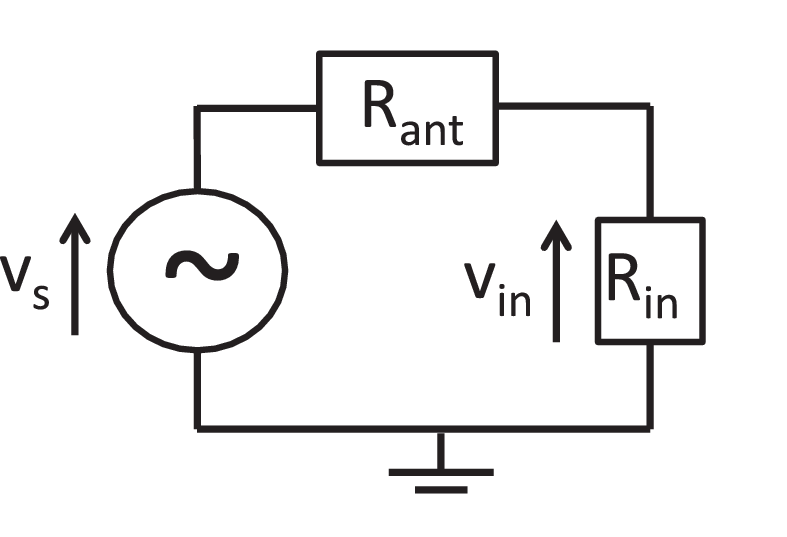
\includegraphics[width=0.48\textwidth]{antenna_equivalent_circuit}\label{fig:antenna_equivalent_circuit}}
  \caption{Rectenna architecture \cite{Clerckx2016}}
  \label{fig:rectenna_architecture}
\end{figure}

Fig. \ref{fig:antenna_equivalent_circuit} illustrates the antenna equivalent circuit. It includes a voltage source ${v_{\text{s}}}(t)$ connected to a series antenna impedance ${Z_{{\text{ant}}}} = {R_{{\text{ant}}}} + j{X_{{\text{ant}}}}$, followed by a combined impedance of the rectifier and the matching network ${Z_{{\text{in}}}} = {R_{{\text{in}}}} + j{X_{{\text{in}}}}$. Assuming lossless, the perfect matching condition is

\begin{equation}\label{eqn:perfect_match}
  {R_{{\text{in}}}} = {R_{{\text{ant}}}},{X_{{\text{in}}}} =  - {X_{{\text{ant}}}}
\end{equation}

When \eqref{eqn:perfect_match} is satisfied, the rectifier input voltage equals

\begin{equation}\label{eqn:rectifier_input_voltage}
  {v_{{\text{in}}}}(t) = {v_{\text{s}}}(t)/2 = y(t)\sqrt {{R_{{\text{in}}}}}
\end{equation}

where ${y(t)}$ is the received signal. Therefore, the input power to the rectifier is

\begin{equation}\label{eqn:rectifier_input_power}
  P_{{\text{rf}}}^r = \mathbb{E}\left[ {y{{(t)}^2}} \right] = \mathbb{E}\left[ {{v_{{\text{in}}}}{{(t)}^2}} \right]/{R_{{\text{in}}}}
\end{equation}

It is also assumed that the noise is too small to be harvested.



\subsection{Diode Characteristics}\label{sec:diode-characteristics}
Consider the single diode rectifier presented in Fig. \ref{fig:single_diode_rectifier} for simplicity. Without loss of generality, the diode models can be employed for other circuits as voltage doubler and bridge rectifiers \cite{Clerckx2017}.

Denoting ${v_{{\text{in}}}}(t)$ and ${v_{{\text{out}}}}(t)$ as diode input and output voltages, the voltage across the diode is ${v_{\text{d}}}(t) = {v_{{\text{in}}}}(t) - {v_{{\text{out}}}}(t)$. It determines the current flowing through the diode

\begin{equation}\label{eqn:diode_characteristics}
  {i_{\text{d}}}(t) = {i_{\text{s}}}\left( {{e^{\frac{{{v_{\text{d}}}(t)}}{{n{v_{\text{t}}}}}}} - 1} \right)
\end{equation}

where ${i_{\text{s}}}$ is the reverse saturation current, $n$ is the ideality factor, and ${{v_{\text{t}}}}$ is the thermal voltage. With Taylor expansion around a quiescent point $a = {v_{\text{d}}}(t)$, equation \ref{eqn:diode_characteristics} rewrites as

\begin{equation}\label{eqn:diode_current_expansion}
  {i_{\text{d}}}(t) = \sum\limits_{i = 0}^\infty  {k_i^\prime } {\left( {{v_{\text{d}}}(t) - a} \right)^i}
\end{equation}

with

\begin{equation}\label{eqn:diode_k_prime}
  k_i^\prime  = \left\{ {
  \begin{array}{*{20}{c}}
    {{i_{\text{s}}}\left( {{e^{\frac{a}{{n{v_{\text{t}}}}}}} - 1} \right),}&{i = 0} \\
    {{i_{\text{s}}}\frac{{{e^{\frac{a}{{n{v_{\text{t}}}}}}}}}{{i!{{\left( {n{v_{\text{t}}}} \right)}^i}}},}&{i \in {\mathbb{N}^ + }}
  \end{array}} \right.
\end{equation}


$k_i^\prime $ depends on the diode parameters and is a constant when $a$ is fixed. Note that the Taylor series expression is a small-signal model that only fits the nonlinear operation region of the diode. Therefore, \eqref{eqn:diode_current_expansion} is no longer accurate for a large input voltage ${v_{{\text{in}}}}(t)$, where the diode behavior is dominated by the series resistor and the I-V relationship is linear \cite{Boaventura2013}.

Also, we assume an ideal rectifier with steady-state response to deliver a constant output voltage ${v_{{\text{out}}}}$, whose amplitude is a function of the peaks of the input voltage ${v_{{\text{in}}}}(t)$ \cite{Curty2005}. Based on those assumptions, a proper choice of voltage drop would be

\begin{equation}\label{eqn:diode_voltage_drop}
  a = \mathbb{E}\left[ {{v_{\text{d}}}(t)} \right] = \mathbb{E}\left[ {{v_{{\text{in}}}}(t) - {v_{{\text{out}}}}} \right] =  - {v_{{\text{out}}}}
\end{equation}

On top of \eqref{eqn:diode_voltage_drop} and \eqref{eqn:rectifier_input_voltage}, the diode current \eqref{eqn:diode_current_expansion} can be further expressed as

\begin{equation}\label{eqn:diode_current}
  {i_{\text{d}}}(t) = \sum\limits_{i = 0}^\infty  {k_i^\prime } {v_{{\text{in}}}}{(t)^i} = \sum\limits_{i = 0}^\infty  {k_i^\prime } R_{{\text{ant}}}^{i/2}y{(t)^i}
\end{equation}

It reveals an explicit relationship between the received waveform $y(t)$ and the diode current ${i_{\text{d}}}(t)$. Nevertheless, the waveform varies at every symbol period due to the randomness of the input distribution. Hence, the diode current ${i_{\text{d}}}(t)$ also fluctuates with time. By taking an expectation over the symbol distribution, the harvested DC current can be modeled as

\begin{equation}\label{eqn:diode_current_expectation}
  {i_{{\text{out}}}} = \mathbb{E}\left[ {{i_{\text{d}}}(t)} \right]
\end{equation}

so the available power is

\begin{equation}\label{eqn:harvested_power}
  P_{{\text{dc}}}^r = i_{{\text{out}}}^2{R_{\text{L}}} = \mathbb{E}{\left[ {{i_{\text{d}}}(t)} \right]^2}{R_{\text{L}}}
\end{equation}

To investigate the fundamental dependency of harvested power on waveform design, a practical strategy is to approximate \eqref{eqn:diode_current} with truncation to the ${n_o}$-th order

\begin{equation}\label{eqn:output_current_truncation}
  {i_{{\text{out}}}} \approx \sum\limits_{i = 0}^{{n_o}} {k_i^\prime } R_{{\text{ant}}}^{i/2}\mathbb{E}\left[ {y{{(t)}^i}} \right]
\end{equation}

The contribution of odd terms is indeed zero as $\mathbb{E}\left[ {y{{(t)}^i}} \right] = 0$ for odd $i$. Therefore, the approximated rectifier output DC current equals

\begin{equation}\label{eqn:output_current_function}
  {i_{{\text{out}}}} \approx \sum\limits_{i{\text{ even,i}} \geqslant 0}^{{n_o}} {k_i^\prime \left( {{i_{{\text{out}}}}} \right)} R_{{\text{ant}}}^{i/2}\mathbb{E}\left[ {y{{(t)}^i}} \right]
\end{equation}

Recall from \eqref{eqn:diode_k_prime} that the diode parameter $k_i^\prime $ is a function of $a =  - {v_{{\text{out}}}} =  - {i_{{\text{out}}}}{R_{\text{L}}}$. Therefore, ${i_{{\text{out}}}}$ occur in both sides of \eqref{eqn:output_current_function}. \cite{Clerckx2016} suggested an approach to decouple the correlation. Denote

\begin{equation}\label{eqn:diode_k_prime_prime}
  k_0^{\prime \prime } = {e^{\frac{a}{{n{v_{\text{t}}}}}}} = {e^{ - \frac{{{R_{\text{L}}}{i_{{\text{out}}}}}}{{n{v_{\text{t}}}}}}}
\end{equation}

such that $k_0^\prime  = {i_{\text{s}}}(k_0^{\prime \prime } - 1)$ and \eqref{eqn:output_current_function} rewrites as

\begin{equation}\label{eqn:output_current_rewritten}
  {e^{\frac{{{R_{\text{L}}}{i_{{\text{out}}}}}}{{n{v_{\text{t}}}}}}}\left( {{i_{{\text{out}}}} + {i_{\text{s}}}} \right) \approx {i_{\text{s}}} + \sum\limits_{i{\text{ even}},i \geqslant 2}^{{n_o}} {\frac{{k_i^\prime }}{{k_0^{\prime \prime }}}} R_{{\text{ant}}}^{i/2}\mathbb{E}\left[ {y{{(t)}^i}} \right]
\end{equation}

Note the r.h.s. of \eqref{eqn:output_current_rewritten} is independent of ${i_{{\text{out}}}}$. On the other hand, the l.h.s. is a monotonic increasing function of ${i_{{\text{out}}}}$. Therefore, we can further write

\begin{equation}\label{eqn:diode_k}
  {k_i} = \frac{{k_i^\prime }}{{k_0^{\prime \prime }}} = \frac{{{i_{\text{s}}}}}{{i!{{\left( {n{v_{\text{t}}}} \right)}^i}}}
\end{equation}

Therefore, maximizing ${i_{{\text{out}}}}$ is equivalent to maximizing the target function

\begin{equation}\label{eqn:target_function}
  {z_{DC}} = \sum\limits_{i{\text{ even,i}} \geqslant 2}^{{n_o}} {{k_i}} R_{{\text{ant}}}^{i/2}\mathbb{E}\left[ {y{{(t)}^i}} \right]
\end{equation}
